%%
%% This is file `sample-acmsmall-conf.tex',
%% generated with the docstrip utility.
%%
%% The original source files were:
%%
%% samples.dtx  (with options: `acmsmall-conf')
%% 
%% IMPORTANT NOTICE:
%% 
%% For the copyright see the source file.
%% 
%% Any modified versions of this file must be renamed
%% with new filenames distinct from sample-acmsmall-conf.tex.
%% 
%% For distribution of the original source see the terms
%% for copying and modification in the file samples.dtx.
%% 
%% This generated file may be distributed as long as the
%% original source files, as listed above, are part of the
%% same distribution. (The sources need not necessarily be
%% in the same archive or directory.)
%%
%%
%% Commands for TeXCount
%TC:macro \cite [option:text,text]
%TC:macro \citep [option:text,text]
%TC:macro \citet [option:text,text]
%TC:envir table 0 1
%TC:envir table* 0 1
%TC:envir tabular [ignore] word
%TC:envir displaymath 0 word
%TC:envir math 0 word
%TC:envir comment 0 0
%%
%%
%% The first command in your LaTeX source must be the \documentclass
%% command.
%%
%% For submission and review of your manuscript please change the
%% command to \documentclass[manuscript, screen, review]{acmart}.
%%
%% When submitting camera ready or to TAPS, please change the command
%% to \documentclass[sigconf]{acmart} or whichever template is required
%% for your publication.
%%
%%
\documentclass[acmsmall]{acmart}

%%
%% \BibTeX command to typeset BibTeX logo in the docs
\AtBeginDocument{%
  \providecommand\BibTeX{{%
    Bib\TeX}}}



%%
%% Submission ID.
%% Use this when submitting an article to a sponsored event. You'll
%% receive a unique submission ID from the organizers
%% of the event, and this ID should be used as the parameter to this command.
%%\acmSubmissionID{123-A56-BU3}

%%
%% For managing citations, it is recommended to use bibliography
%% files in BibTeX format.
%%
%% You can then either use BibTeX with the ACM-Reference-Format style,
%% or BibLaTeX with the acmnumeric or acmauthoryear sytles, that include
%% support for advanced citation of software artefact from the
%% biblatex-software package, also separately available on CTAN.
%%
%% Look at the sample-*-biblatex.tex files for templates showcasing
%% the biblatex styles.
%%

%%
%% The majority of ACM publications use numbered citations and
%% references.  The command \citestyle{authoryear} switches to the
%% "author year" style.
%%
%% If you are preparing content for an event
%% sponsored by ACM SIGGRAPH, you must use the "author year" style of
%% citations and references.
%% Uncommenting
%% the next command will enable that style.
%%\citestyle{acmauthoryear}


\usepackage{bussproofs}
\usepackage{proof}
\usepackage{algorithm}
\usepackage[noend]{algpseudocode}
\usepackage[toc]{glossaries}
\usepackage{glossary-mcols}
\usepackage{soul}

\theoremstyle{definition}
\newtheorem{definition}{Definition}[section]
\loadglsentries{terminology}

% For comment boxes.
\usepackage[colorinlistoftodos,prependcaption,textsize=tiny]{todonotes}
\newcommand{\giselle}[1]{\todo[linecolor=red,backgroundcolor=red!25,bordercolor=red]{G: #1}}
\newcommand{\samar}[1]{\todo[linecolor=blue,backgroundcolor=blue!25,bordercolor=blue]{S: #1}}

\newcommand{\dio}{\textsc{dio}}

%%
%% end of the preamble, start of the body of the document source.
\begin{document}


%%
%% The "title" command has an optional parameter,
%% allowing the author to define a "short title" to be used in page headers.
\title{Domain Informed Oracle for Reinforcement Learning}

%%
%% The "author" command and its associated commands are used to define
%% the authors and their affiliations.
%% Of note is the shared affiliation of the first two authors, and the
%% "authornote" and "authornotemark" commands
%% used to denote shared contribution to the research.
\author{Samar Rahmouni}
\email{srahmoun@andrew.cmu.edu}
\orcid{1234-5678-9012}
\affiliation{%
  \institution{Carnegie Mellon University}
  \city{Doha}
  \country{Qatar}
}

\author{Giselle Reis}
\email{giselle@cmu.edu}
\orcid{0000-0002-5145-9829}
\affiliation{%
  \institution{Carnegie Mellon University}
  \city{Doha}
  \country{Qatar}
}



%%
%% By default, the full list of authors will be used in the page
%% headers. Often, this list is too long, and will overlap
%% other information printed in the page headers. This command allows
%% the author to define a more concise list
%% of authors' names for this purpose.
%\renewcommand{\shortauthors}{Trovato et al.}

%%
%% The abstract is a short summary of the work to be presented in the
%% article.
\begin{abstract}
  \giselle{Abstract should be shorter. I crossed out what could be
  removed to achieve this.}
  %% The story

  %% There is this great new method!
  Reinforcement learning (RL) is a powerful AI
  \st{method}{\color{blue}technique} that does not
  require pre-gathered data but relies on a trial-and-error process
  for the agent to learn. 
  %
  This is made possible through a reward function that associates
  \st{current} state configurations to a numerical value. 
  %
  The agent's goal is \st{then} to maximize its cumulative reward over its
  lifetime. 
  % 
  %% Oh, but there are some issues...
  Unfortunately, there is no systematic method to design a reward
  function{\color{blue}, since interpreting abstract states in RL in
  the context of a domain needs to be done on a case by case basis.}
  %
  \st{This needs to be done on a case by case basis, and might be hard
  depending on how the states are represented.}
  %
  \st{States are typically represented as vectors of values in RL, and
  translating properties and rules from a domain into this
  representation can be complicated depending on how many values are
  used, what they represent, whether they are normalized or not,
  etc.}\giselle{This can be elaborated in the introduction.}


%  \medskip

  % This is needed to connect the ideas from the previous paragraph
  % and the next.

%%   %% No problem, we can solve them!
%%   These challenges can be alleviated for a given domain by fine
%%   tuning the reward function with domain specific information. 
%%   %
%%   For example, if the agent is a self-driving car, the reward function
%%   can include the physics equations to predict, with some degree of
%%   certainty, the car's trajectory for the next few seconds.
%%   %
%%   By looking into the future, the reward function can penalize bad
%%   behavior before it reaches a catastrophic state (\emph{e.g.}, a
%%   crash).
%%   %
%%   A better reward function prunes the (often infinite) search space
%%   faster, allowing the agent to explore (breadth) new states instead
%%   of exploiting (depth) dead ends.
%%   %
%%   %% Oh, but only on a case by case basis...
%%   However, tuning the reward might be hard depending on the domain and
%%   how states are represented.
%%   %
%%   States are typically represented as vector of values in RL, and
%%   translating properties and rules from a domain into this
%%   representation can be complicated depending on how many values are
%%   used, what they represent, whether they are normalized or not, etc.

%  \medskip

  %% We can fix that!
  We propose a \emph{Domain Informed Oracle (\dio{})} \st{as a
  solution for}{\color{blue}to}
  systematically incorporat\st{ing}{\color{blue}e} domain specific knowledge into RL
  reward functions.
  %
  \dio{} is a collection of domain specific rules written in a
  declarative language, such as Prolog.
  %
  It does not rely on the RL representation of states, allowing the
  programmer to focus on the domain \st{specific} knowledge using an
  expressive and intuitive language, where \st{they can define states and
  rules in the most convenient way.}{\color{blue}states and rules can
  be defined conveniently.}
  %
  {\color{blue}For each state and action pair,} \dio{} provides
  {\color{blue}information} \st{an informed decision} to the reward
  function, {\color{blue}to dynamically adapt itself} \st{thus
  allowing it to dynamically adapt the rewards}.
  %
  %DIO is incorporated into a RL architecture and is defined by its
  %behavior in relation to the input given by the reward function. 
  
  Our implementation is tested on a grid world with dynamic obstacles.
  \st{and later extended 
  to a traffic simulation scenario. It is then} {\color{blue}and}
  compared to a basic \st{uninformed} RL algorithm. 
  %
  \st{The comparison is based on performance which we define by three
  metrics: time to train, optimality of the learned policy and
  finally, the success percentage, i.e. the number of times it reaches a positive terminal state, a goal 
  for example. }\giselle{This can be elaborated in the experiments
    section.}
  %
  {\color{blue}The results show that the domain specific knowledge
  incorporated easily through \dio{} lead to shorter training times,
  faster convergence, and fewer errors.}\giselle{Specullation...
  Rewrite once results are in.}
  
  \st{Our results show that although the time to train is longer, the
  learned policy using \dio{} succeeds in 90\% of the time to reach
  the goal. The policy both incorporates safety by avoiding crashing
  into an obstacle but also optimality by choosing the fastest
  possible path. This is not the case with an implementation that only
  makes use of RL, precisely a proximal policy optimization that does
  learn safety but always ends its episode in the maximum number of
  steps, rather than reaching the goal.}\giselle{I think this is not
  updated...}

\end{abstract}

%%
%% The code below is generated by the tool at http://dl.acm.org/ccs.cfm.
%% Please copy and paste the code instead of the example below.
%%
\begin{CCSXML}
  <ccs2012>
     <concept>
         <concept_id>10003752.10003790.10003795</concept_id>
         <concept_desc>Theory of computation~Constraint and logic programming</concept_desc>
         <concept_significance>300</concept_significance>
         </concept>
   </ccs2012>
\end{CCSXML}
  
\ccsdesc[300]{Theory of computation~Constraint and logic programming}

%%
%% Keywords. The author(s) should pick words that accurately describe
%% the work being presented. Separate the keywords with commas.
\keywords{probabilistic logic programming, reinforcement learning, reward shaping}
%% A "teaser" image appears between the author and affiliation
%% information and the body of the document, and typically spans the
%% page.

\received{20 February 2007}
\received[revised]{12 March 2009}
\received[accepted]{5 June 2009}

%%
%% This command processes the author and affiliation and title
%% information and builds the first part of the formatted document.
\maketitle

\section{Introduction}

Implementing a robust adaptive controller that is effective in terms
of precision, time, and quality of decision in dynamic and uncertain
scenarios has always been a central challenge in AI and robotics. When
autonomous agents are deployed in the real world, we want to ensure
that they are able to adapt to unforeseen scenarios, as well as keep
their efficiency. This efficiency is measured in terms of optimality
of actions and time to make a decision. 
%
As autonomous cars are deployed, IoT is popularized, and human-robot
interactions become more complex, we are more and more confronted with
the need for robotic agents that can effectively and continually adapt
to their surroundings, not only in simulation, but also in practice,
when deployed as a cyber-physical system.\giselle{Potential to recover
space.}
Since we are unable to
provide a repertoire of all possible scenarios and actions, agents
need to be able to autonomously predict and adapt to changes.
Reinforcement Learning (RL) is an approach that supports dynamically
adapting to new input~\cite{sutton2018reinforcement}. It has beed
successfully used by AlphaGo, Deepmind AlphaStar, and OpenAI Five to
solve Go, StarCraft II and Dota 2~\cite{li2019reinforcement}.

Reinforcement Learning is a powerful tool as it does not require
pre-gathered data as most Machine Learning (ML) techniques do. 
%
The general idea of RL is learning via trial-and-error, guided by a
\textit{domain dependent} reward function.
%
For example, if the agent is a self-driving car, the reward function
would greatly penalize states where it crashes.
%
However, this means that the car is bound to crash to learn not to
crash again.
%
A better reward function can include the physics equations to predict,
with some degree of certainty, the car's trajectory for the next few
seconds.
%
By looking into the future, the reward function can penalize bad
behavior before it reaches a catastrophic state (a crash).
%
A better reward function prunes the (often infinite) search space
faster, allowing the agent to explore (breadth) new states instead of
exploiting (depth) dead ends.
%
%For example, say we want to teach an autonomous car to stop at a STOP
%sign. We will punish it via a negative reward when it does not,
%otherwise, we will reward it. Thus, through multiple iterations, and
%with the goal to maximize its rewards, a reinforcement learning
%trained agent will learn to stop at a STOP sign. 

The task of choosing the reward function is thus crucial.
{\color{blue}The natural follow up to this sentence would be the
argument of why desinging the function is hard. I think the motivation
section is a nice continuation, and I would perhaps even have it as a
subsection of the introduction. Alternatively, end the introduction
with the part below, and keep the motivation section.}
%
In this work, we propose a Domain Informed Oracle (\dio{}) written in a
declarative language to inform a reinforcement learning algorithm. 
%
Our method provides a systematic way to encode domain specific rules
into a reward function for RL that does not rely on the state
representation within the RL algorithm.
%
\st{We argue that such a combination will ensure a faster and more
efficient RL trained agent in terms of optimality. 
%
The proposed combination is tested on a traffic simulation and the
results are compared with a RL implementation that makes use of
standard practices to design a reward function. }\giselle{Parts of
this can be used to rephrase things in the abstract.}

%%
%% Our motivation from the lack of symbolic reasoning
%% to inform a reinforcement learning modules
%% The challenges of finding a 'good' reward function
%%
\section{Motivation} 

Reinforcement Learning is a method of learning that maps situations to
actions in order to maximize its rewards
\cite{sutton2018reinforcement}. Rewards are numerical values associated to a state and action. Precisely, one defines a reward function 
$R : (S \times A) \rightarrow \mathbb{R}$ where $S$ defines the state space and $A$ the action space. Note that a state refers to the current configuration
of the environment and the action refers to the action chosen by the RL agent. By defining this reward function and the scenario of the problem the agent is trying to solve, 
reinforcement learning has the advantage of not requiring a prior dataset. Indeed, the agent is not told what to do, but rather 
learns from the effect of its actions on the environment. 
% Consider Figure~\ref{fig:rl}. [GR] You are explaining the figure in
% the next paragraph, so this sentence is not needed.

\begin{figure}[H]
  \centering
  
\includegraphics[scale=0.6]{figures/rlroutine.png}
  \caption{Reinforcement Learning Routine}
  \label{fig:rl}
\end{figure}


The diagram in Figure~\ref{fig:rl} is a high-level description of how
an agent using reinforcement learning can be trained.  
%
The upper left box represents the \emph{environment} as seen by the agent
according to its sensors.
%
The current state of the environment is represented as a \emph{state
vector}.
%
At each iteration, the agent will receive the state vector as input,
and needs to choose an \emph{action} to take.
%
Once the action is taken, the environment is updated to the next state
and the agent receives a \emph{reward} as feedback.
%
This reward is a domain dependent function that represents how
``good'' the new state is.
%
The agent's goal is to increase its reward by taking actions that
reach better states each time.
%
The triple (state, action, reward) helps the agent in shaping the
final policy.

\medskip 

The reward function is a crucial aspect of the RL algorithm. For instance, consider a game of chess 
where the agent is punished when it loses and rewarded if it wins. The agent is bound to learn how to 
maximize its winnings but it will need to exhaust multiple possible combinations to learn. In this case, 
the training time is not optimal. A better approach would be to also reward it for making a good opening, for instance. 
Another example would be only considering negative rewards. Say we want our agent to escape a maze, and we punish it at every timestep for not escaping. 
If there is a fatality state (\emph{e.g.}, a fire or a black whole), the agent will learn to move towards the fatality state as to cut its negative rewards as soon as possible. 
In conclusion, a good reward function is the first step of optimal learning. By choosing the right reward function, 
we can ensure a faster and more efficient training, possibly with fewer errors. 

For more information on the algorithms we have used for our implementations, refer to \ref{sec:rldetails}.

\subsection{Challenges in Reinforcement Learning}
\label{sec:challenges}

Reward shaping (1), the exploration-exploitation dilemma (2) and
meta-learning (3) are main challenges
that make it harder for RL to be adopted as a solution to more real-world problems. 

\medskip 

\emph{Reward shaping}~\cite{laud2011} refers to the lack of systematic methods to design a reward
  function that ensures fast and efficient learning. This generation of an appropriate 
reward function for a given problem is still an open challenge~\cite{kober2013}.
Ideally, rewards would be given by the real-world, i.e. \textit{native rewards}. For instance, recent work investigates dynamically generating a reward 
using a user verbal feedback to the autonomous agent~\cite{gonzalez2010}. However, most RL agents 
can only stay in simulation due to the lack of safety guarantees. This is because of the trial-and-error nature of the RL training. 
Thus, there exists a need for \textit{shaping rewards} instead. There are reasonable criteria on how this should be done, those are \emph{standard practices}. For instance, 
rewards that can be continuously harvested speed up convergence
compared to rewards that can only be harvested at ``the end''
(\emph{i.e.} the chess example). Similarly, one should avoid only 
negative rewards as that results in unwanted behavior. Furthermore, if dealing with a continuous state space, it helps to have a polynomial differential function as the reward function 
as it is shown to help the agent learn faster. Finally, one can normalize rewards at the end as to not end up with too many discrepancies. 
However, there still exists a lack of a systematic method to design a
reward function, and this needs to be done on a case by case basis.
%
\dio{} does not rely on an abstract representation to infer a reward function, rather only needs 
to care about the translation to a domain specific language, like prolog or datalog to assess a given world. 
It provides a more declarative approach to reason about rewards, thus providing a systematic method to map 
labels to rewards. As a consequence, it is able to handle (2), namely, the exploitation vs. exploration
dilemma.

\medskip

The \emph{exploration vs. exploitation dilemma} is the question of whether to always exploit what the
agent knows or explore in the hope that an unexplored state might
result in better rewards. This dilemma of \emph{exploration} vs. \emph{exploitation} is a central issue of RL. Consider this problem. An agent is at an intersection. It has the choice of going either right or left. 
It does not yet know the outcome of either. It chooses right at a given point and receives a reward $r=1$. The question is "When faced with the same decision, should it keep going right?" There are two issues to consider. 
First, it does not know the outcome of going left. It could be that there is a better reward waiting for it on the left lane. Second, when dealing with a stochastic environment, it might be that $r$ was a one-time occurence. 
It would be equivalent to someone buying a lottery ticket, and winning
\$1M on their first try, and thus, spending all that they won in trying to make it happen again. This problem showcases the importance of exploration; an agent 
needs to see where other paths might lead to, but also exploitation; if it keeps exploring forever it will never accumulate rewards. This is especially evident when the possible states cannot be exhausted. Several techniques have been proposed 
to balance between exploration and exploitation \cite{Kaelbling1996ReinforcementLA}. A notable one is the \emph{epsilon-greedy} technique. The idea is to set some probability $\epsilon$ by which the agent decides to explore. This probability can be adapted 
to decrease as more \emph{episodes} are completed. However, by ensuring (1), an informed reward function is able to sufficiently 
deter the exploration of undesirable states while encourage the exploitation of desirable ones, continuously adapting to 
acquired knowledge and resolving the conflict when necessary. More interestingly, a solution to (2) impacts (3). 


\medskip

\emph{Meta-learning} is the problem of deploying an agent trained in a simulation to
the real-world, or possibly another simulation, where it encounters
state configurations it did not during its training. The goal is to
be able to efficiently adapt to those configurations. The problem of meta-learning in RL stems from the uncertainties of the world. 
Consider the result of training: a function $\pi$ that map states to
actions $\pi : S \rightarrow A$. The learned policy is the one that maximizes the cumulative rewards.
This training is most often done in simulation, given the lack of safety guarantees of RL. 
However, several problems come into place when considering the deployment of the trained agent. Considering that an agent has done well in 
a designated simulation does not imply that it will do as well in the real-world. Overall, it must be that certain uncertainties will not be expected, thus there can be no expectation on how the agent will behave 
when out of simulation. Meta-learning in reinforcement learning is the problem of learning-to-learn, which is about efficiently
adapting a learned policy to conditions and tasks that were not encountered in the past. In RL, meta-learning
involves adapting the learning parameters, balancing exploration and exploitation to direct the
agent interaction \cite{gupta_meta-reinforcement_2018,schweighofer_meta-learning_2003}. Meta-learning is a central problem in AI, since an agent that can solve more
and more problems it has not seen before, approaches the ideal of a general-purpose AI. However, as noted previously, a solution to (2) implies 
a continuous adaptation to knowledge. Since the conflict of exploration and exploitation is resolved, the agent adapts accordingly to tasks it encountered in the past (exploiting), but also 
tasks it encounters for the first time (exploring). Thus, from (2) one
can have a significant impact on (3).


\subsection{Symbolic Reasoning for Reinforcement Learning} 
\label{symrl}

To tackle the challenges from Section~\ref{sec:challenges}, we are
inspired by the current Neurosymbolic AI trends, which explore
combinations of deep learning (DL) and symbolic reasoning.
%
The work has been a response to criticism of DL on its lack of formal
semantics and intuitive explanation, and the lack of expert knowledge
towards guiding machine learning models.
%
A key question the field targets is identifying the necessary and
sufficient building blocks of AI~\cite{garcez2020neurosymbolic},
namely, how can we provide the semantics of knowledge, and work
towards meta-learning? 
%
Current Neurosymbolic AI trends are concerned with knowledge representation and reasoning, namely, they investigate computational-logic systems 
and representation to precede learning in order to provide some form
of incremental update, e.g. a meta-network to group two sub-neural
networks~\cite{Besold2017NeuralSymbolicLA}.
As a result, neurosymbolic AI has been successfully applied to vision-based tasks such as semantic labeling \cite{vinyals2015, karpathy2015}, 
vision analogy-making \cite{Reed2015DeepVA}, or learning communication
protocols \cite{Foerster2016LearningTC}.
Those results inspire us to use those techniques for reinforcement learning, as to tackle its challenges.


%%
%% What is it that we propose? 
%% Domain Informed Oracle! A logic programming module to 
%% inform a reinforcement learning module through reward-shaping
%%
\section{Domain Informed Oracle} 

We tackle the challenge of finding a systematic method to map a state to a numerical value: a reward. 
To do so, we make use of the fact that rewards are domain dependent and thus, given domain specific rules, a \emph{domain informed} module can guide a RL agent towards better decisions. This can be done by 
adapting the reward function. For instance, we consider defining which states are desirable, which are to be avoided and which are fatal. Given rules and judgments, a logic programming module 
is able to search the space and send feedback to the reinforcement learning agent. The goal is a systematic method to design a reward function which can ensure faster and more efficient 
training. This knowledge can furthermore be incorporated into resolving the exploration vs. exploitation dilemma. For instance, if a domain informed module 
can infer that only one of the possible next states is desirable, then exploration in that specific case is suboptimal.  
We will call the proposed module a \emph{Domain Informed Oracle}
(\dio{}).

\begin{figure}[H]
  \centering
  
\includegraphics[scale=0.45]{figures/overview.png}
  \caption{Overview of the proposed solution}
  \label{fig:overview}
\end{figure}


The diagram in Figure~\ref{fig:overview} is a high-level description of our proposed solution. 
%
Precisely, the (state, action) pair is fed into \dio{}. While the environment produces its own 
reward function, \dio{} also computes its own reward. 

We could leave the \emph{reward shaping} unit as a design choice.
However, it will be argued in~\ref{sec:comreward}
that whether it is left as a design choice or else, is irrelevant given how \dio{} affects the final results.

\subsection{Architecture}
In this section, we lay the foundations of the architecture that combines the Domain Informed Oracle with 
reinforcement learning. Note that in our proposed architecture, we suppose Proximal Policy Optimization~\cite{schulman17ppo}. 
It does not mean that our solution is specific to it, rather it can be generalized to any algorithm choice.

\begin{figure}[H]
  \centering
  \begin{minipage}{.5\textwidth}
    \centering
    
\includegraphics[width=1\linewidth]{figures/basicrl.png}
    \captionof{figure}{Reinforcement learning architecture}
    \label{fig:basicrl}
  \end{minipage}%
  \begin{minipage}{.45\textwidth}
    \centering
    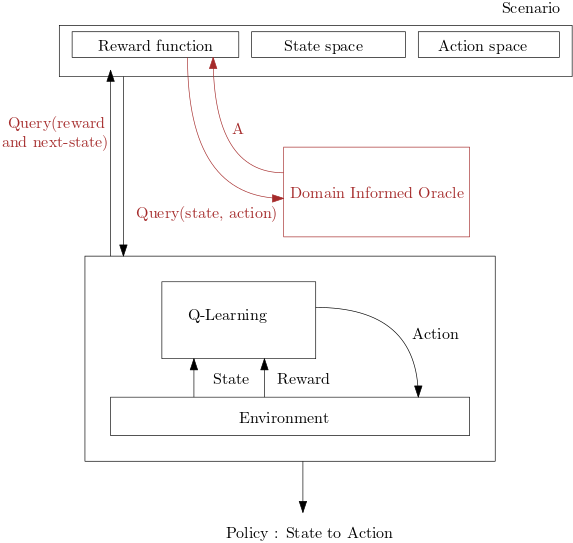
\includegraphics[width=1\linewidth]{figures/dio.png}
    \captionof{figure}{\dio{}+RL architecture}
    \label{fig:diorl}
  \end{minipage}
\end{figure}\giselle{There are some labels missing in
Figure~\ref{fig:basicrl}, and I think an arrow from the scenario box
to the RL box in Figure~\ref{fig:diorl}.}

The diagram in Figure \ref{fig:basicrl} describes the basic routine of RL in more detail. The environment defined by the scenario sends the current state 
to the \emph{Proximal Policy Optimization} algorithm. The agent chooses an action from the action space and sends it to the environment. This action affects the environment stepping it to some next state. 
The resulting state along its associated reward is computed from the reward function and step function formalized in the scenario. Thus, in the next iteration, the 
agent receives the reward from its previous action which it uses to improve its policy and continues with its training starting from the computed next state.  

The architecture in Figure \ref{fig:diorl} introduces \dio{} in the feedback loop. It is kept independent of the RL module. Precisely, when the scenario is query-ed for the reward and 
the resulting next state of a (state, action) pair, rather than
computing the reward using the reward function, the latter is able to
query \dio{}. The result of this query is $J$\giselle{Is this $A$ in
the figure?}: a numerical value 
we defined as $r_\dio{}$, the reward given by \dio{} to the (state, action) pair. More on how this reward is computed in \ref{sec:comreward}.
 

\subsection{\dio{} procedure}
\label{sec:modules}
In practice, we consider the following modules and their interactions as shown in \ref{fig:mods}.


\begin{multicols}{2}
\begin{enumerate}
  
  \item \textbf{World Rules} defining the rules governing the world. This is domain-dependent and implemented 
        in a logic programming file, i.e. we are able to define the next step via step semantics.
  
  \item \textbf{Knowledge Base} defining the ground facts which describe the world at a given time step. This module is 
        continuously updated to account for the dynamics of the
        state.

  \item \textbf{Labels} i.e., textual ``norms'' corresponding to an
  iteration of the state. In practice, they are all possible judgments
  on the resulting state, e.g. \textit{crash :- obs(X,Y), agent(X,Y)},
  or \textit{maybecrash :- nextObs(X,Y), agent(X,Y)}.  Those labels
  have probabilities associated with them and indicators. Precisely,
  an indicator over a negative state is $-1$. 

  \item \textbf{Translation Unit} defining the translation from state
  to ground facts and from labels to a numerical value, e.g. if the
  predicate crash is true with $P = 0.25$, then the reward shaped is
  $r + (-0.25)$.

  \item \textbf{Reinforcement Learning} is our independent module that
  does not make assumption on the algorithm chosen for RL.
\end{enumerate}
\end{multicols}


\begin{figure}[H]
  \centering
  
\includegraphics[scale=0.4]{figures/dynamics.png}
  \caption{Modules \& Interactions}
  \label{fig:mods}
\end{figure}

Figure \ref{fig:mods} describes the interactions of the different
modules. Precisely, given the rules and the world knowledge base at a
given time $t$, we are able to produce the corresponding label, i.e.
the query over a predicate. The predicate is fed into the Translation
Unit (TU) that transforms the predicate to a numerical value that is
given to the Reinforcement Learning as a reward shaping $r'$. Note
that the inference on the query is done by a declarative tool that
incorporates probabilities called \emph{Problog} that we introduce in
\ref{sec:problog}.


\subsection{Problog Procedure} 
\label{sec:problog}
% High level overview of Problog
Problog is a logic programming language that aims to bridge between probabilistic 
logic programming and statistical relational learning \cite{fierens_van}. 

\begin{definition}[Statistical Relational Learning (SRL)]
    Discipline of Artificial Intelligence that considers first order logic relations between 
    structures of a complex system and model it through probabilistic graphs such as Bayesian or 
    Markov networks.
\end{definition}

\begin{definition}{Probabilistic Logic Programming (PLP)}
    Discipline of Programming Languages that augments traditional logic programming such as Prolog 
    with the power to infer over probabilistic facts to support the modeling of structured 
    probability distributions.
\end{definition}

A problog program specifies a probability distribution over possible worlds. 
This probability distribution corresponds to the possible worlds whether a fact is taken 
or discarded given the probability associated with it. Precisely, they define a world 
as a subset of ground probabilistic facts where the probability of the subset is the product of 
the probabilities of the facts it contains.
%
% Evidence and inference tasks in Problog
Furthermore, problog extends PLP with the power of considering evidences 
in the inference task. This is made possible without requiring the transformation 
the Bayesian networks on which to use SRL. Instead, problog considers the subset described above 
and assumes only worlds where the evidence held remains true. Those possible worlds and their associated 
probabilities are then added and divided by the choice with the higher probability. Problog makes this 
possible by a 3-steps conversion from a problog program to a weighted boolean formula.

% Conversion steps to weighted formula
First, problog grounds the program by only considering facts relevant to the query in question. 
The relevant ground rules are specifically converted to equivalent Boolean formulas. 
Precisely, inferences are converted into bi-directional implications and its corresponding premises 
are converted to a conjunction of disjunction of facts. 
Finally, problog asserts the evidence by adding it to the previous boolean formula 
as a conjunction and defines a weight function that assigns a weight to every literal. 
The weights are derived from the probability associated with the relevant literal, whether explicility 
given or implicility computed. 

% How exactly are we getting this numerical value?
\subsection{Computation of Final Reward}
\label{sec:comreward}
In general, reward shaping is expressed as follows
  $R = r_{rl} + r'$, 
such that $r_{rl}$ is the original reward defined by the reinforcement learning environment. Usually, this associates the value of $1$ for a positive terminal state, 
and $-1$ for a negative terminal state. $r'$ is the human bias, i.e.
what is added to ``shape'' the reward function. 
Although only rewarding terminal states is enough to reach a policy
that will minimize its losses, it is important to note that a reward
function should consider the cost of a step 
for optimal and fast training. The cost of a step is dependent on the state given at that step. For instance, an autonomous vehicle stopping with no cars around is different from a vehicle 
stopping while a car is behind it. Although the states are not
\emph{terminal}, i.e. they do not end an episode, they have different weights. 
An optimal reward function is one that considers those differences. A logic programming module allows us to infer over states using a knowledge base and world rules seamlessly. 

Let's consider the following example in Figure~\ref{fig:diospecs}.
Our agent is running away from a predator. It is currently at position $(0,0)$, and decides to go right, to escape. 
Since, it is a stochastic environment, there is a 0.1 chance that his parts might fail and he stays in the same spot, thus getting eaten by the predator. 
This is easily expressed in \emph{problog} as follows. 
\begin{verbatim}
  0.9 :: pos(X+1, Y) :- direction(right), pos(X, Y). 
  0.1 :: pos(X, Y) :- direction(right), pos(X, Y). 
\end{verbatim}
Consequently, there is a 0.9 chance that we end up in a `desirable'
state, and a 0.1 chance that we end up in an `undesirable' state.
Therefore, 
\[ 
   r'_{\dio{}} = \sum_{L} Pr[L \mid (s_t, a_t)] I[L]
\] 

\noindent
where desirable and undesirables are labels noted by $L$. We identify their indicator $I[L]$ by $1$ if positive, $-1$ if negative.
This is equivalent to the expectation over a (state, action) pair computed by the logic programming module. 
\begin{figure}
  \centering
  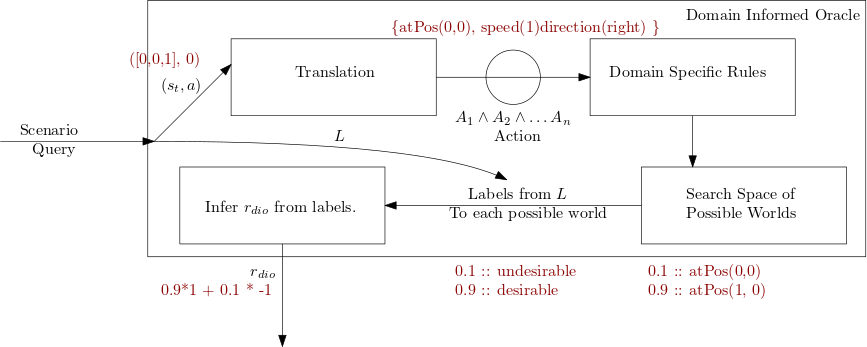
\includegraphics[scale=0.45]{figures/diospecs.png}
  \caption{Step-by-step of Computed Final Reward}
  \label{fig:diospecs}
\end{figure}

It is the case that this reward has to be normalized to the weight of a step. Indeed, suppose there are $S$ possible states for the agent to be at. 
The accumulated reward of the steps should at most equal that of the terminal states. Thus, the final reward, 
\[
  r_{\dio{}} = \dfrac{r'_{\dio{}}}{S} \qquad \text{ and } \qquad
  R = r_{rl} + \alpha r_{\dio{}}
\]
\giselle{Define S}

Note that the final reward from \dio{} is added considering some $\alpha$. This is precisely for comparison purposes, i.e. how much value should we give the logic programming module 
to inform a step. 



%%
%% How would this look in practice?
%% Let's go through our working example. 
%%
\section{Dynamic Obstacles in a GridWorld : Working Example} 
\label{gridworlddyn}

For our experiments, we take the following scenario. An agent exists in a 100x100 grid. 
There are $n$ dynamic obstacles around that have uniform chances of choosing any direction to move in. 
The agent can make a decision to move either right, left, top or bottom, as well as not moving at all. 
There is a goal in the bottom-right of the grid. The agent has two goals: (1) survive by not crashing with the obstacles and (2) reach the goal in the lowest number of steps possible. 

\subsection{Scenario in Reinforcement Learning}

This environment offered by gym-gridworld~\cite{gym_minigrid} is useful for testing our algorithm in a Dynamic Obstacle avoidance for a partially observable 
environment. Precisely, we define the state as follows. 
\begin{equation*}
  S_t = [x, y, d, G]
\end{equation*}
$(x,y)$ define the position of our agent while $d$ its direction. $G$
is the gridworld observed by the agent which includes walls, obstacles
and free squares. Note that this observed environment is from the point of the view 
of the agent and does not represent the entire grid. 
The action space is, 
\begin{equation*}
  A_t = \{ \text{right}: 0, \text{up}: 1, \text{down}: 2, \text{left}: 3 \}
\end{equation*}
Finally, the reward is a straightforward one that reward $1$ for reaching the goal, $-1$ for failing to do so, either by colliding with an obstacle, 
or exhausting its battery (maximum number of steps). Furthermore, for
every step the agent takes, it has to spend the \emph{cost of living},
which is $-1/n$, where $n$ is the size of board.


\subsection{Domain Specific Rules}

The rules are defined in ProbLog~\cite{problog}: a probabilistic prolog that allows us to capture 
the stochasticity of the environment, as we previously introduced in
Section~\ref{sec:problog}. Precisely, we want to consider the erratic movements of the obstacles, considering 
we do not have previous knowledge on the distribution of their given movement. We assume a uniform distribution and define the following. 
The rules of \dio{} deriving a predicate $\gamma$ take the following form: 

\begin{prooftree}
  \AxiomC{$P_1 :: \psi_1$}
  \AxiomC{\dots}
  \AxiomC{$P_n :: \psi_n$}
  %\AxiomC{$\sum_{i=0}^{n}P(i) = 1$}
  \RightLabel{(action)}
  \TrinaryInfC{$Q :: \gamma$}
\end{prooftree}

\noindent
where $Q$ and $P_1, ..., P_n$ are probabilities for the facts $\gamma$
and $\psi_1, ..., \psi_n$, respectively.
%
The rule should be read as an implication from the top down, i.e., if
the premise facts $\psi_1, ..., \psi_n$ hold with their corresponding
probabilities, than we can infer the conclusion $\gamma$ with
probability $Q$.
%
Note that $Q$ will naturally be a function of $P_1, ..., P_n$.
%
If there are $k$ rules with conclusions $Q_1 :: \gamma, ..., Q_k ::
\gamma$, then it must be the case that $\sum_{i=0}^{k} Q_i = 1$.
%, and $\varphi(i)$ corresponds to the conjunction of grounds facts of the possible world with probability $P_i$.
The action is equivalent to our step semantics. 
In the gridworld example, we give the following. 

\vspace{0.2cm}
\begin{center}
  \AxiomC{atPos(X,Y)}
  \AxiomC{speed(V)}
  \AxiomC{timestep(T)}
  \RightLabel{(right)}
  \LeftLabel{(1)}
  \TrinaryInfC{atPos(X + V*T, Y)}
  \DisplayProof
  \hspace{0.2cm}
  %
  \AxiomC{obs(X,Y,V)}
  \AxiomC{timestep(T)}
  \LeftLabel{(2)}
  \RightLabel{(time)}
  \BinaryInfC{0.2 :: obs(X + V*T, Y, V)}
  \DisplayProof
\end{center}
\vspace{0.2cm}

(1) considers the movement of the agent while (2) considers the movement of the obstacles. Note that (2) considers 
a uniform distribution over the movement of the obstacle, since every
obstacle has a uniform probability of moving
up/down/left/right or staying in place.
We could do the same for (1) by considering the probability of an action failing. In our case, we assume the movement is deterministic and no failure over the movement 
of the agent happens.


\subsection{World Knowledge}
Our world knowledge base covers the agent, the obstacles and the timestep. We consider two cases: 
\textit{constant} ground facts vs. \textit{dynamic} ground facts. The latter represents positions which are dynamically 
generated at every timestep while the former considers only the facts that remain true in every world, thus include the timestep, since we always
move by 1-unit, and the speed, since the agent and the obtacles are defined to only move by 1-box every time. Given that our knowledge base $Kb$ is defined by, 
\[
    C = \{\text{speed}(1), \text{timestep}(1) \}     
    \qquad
    D = \{\text{atPos}(X, Y), \text{obs}(X,Y,1)\}
    \qquad
    Kb = C \cup D
\]

\subsection{From Norms to Labels}
In the following, we define \textbf{\glsplural{norms}} as textual sentences to describe the intended goal behavior. 
Thus, in the gridworld example, we consider one possible norm, (1) \textit{crash} when the agent and the obstacle \emph{possibly} overlap. That is if there is a chance of 
the obstacle and the agent choosing to move to the same square. 

\[
    \infer{P_1 \times P_2 :: \text{crash}}{
      P_1::\text{atPos}(X,Y)
      &
      P_2::\text{obs}(X,Y,\_)
      & 
      \ldots}
\] 

Note that the final $P$ associated to our label is exactly $Pr[L \mid (s_t, a_t)]$. 

\subsection{Translation Unit}

The translation unit is the bridge between \dio{} and RL. It handles both feeding 
the world facts to \dio{} and translates the feedback given to a numerical value, through 
a given function. First, the \dio{}/RL loop is given in Algorithm 1. 

  \begin{algorithm}[H]
    \caption{\dio{}/RL Loop}
    \begin{algorithmic}[1]
    
    \Procedure{Step}{$S_t, a$}       \Comment{(State, action) Pair}
        \State Check for invalid actions
        \State Check for obstacles 
        \State Update Obstacles positions
        \State Update Agent's position
        \State \textbf{TU.UpdateWorld}(position, direction, obstacles) \Comment{KB update in \dio{}}
        \State $obs, r_{rl}$ = Step'$(S_t, ac)$ \Comment{Call to Initial Env}
        \State $r_{\dio{}}'$ = \textbf{getFeedback()} \Comment{Query \dio{}}
        \State $R$ = TU.getReward($r_{rl}, r_{\dio{}}'$) 
        \State return (obs, R)
    \EndProcedure
    
    \end{algorithmic}
    \end{algorithm}

Note that the translation unit first updates the knowledge base from \dio{} side. 
Given this update, it is possible to query \dio{} over the labels and their associated probabilities. Precisely, 
the \emph{getFeedback} procedure computes $r'_{\dio{}}$ the expected value over the possible worlds. 

\begin{algorithm}[H]
  \caption{Inference of Judgment $r'_{\dio{}}$}
  \begin{algorithmic}[1]
      
      \Procedure{getFeedback}{} 
      \State labels $\gets$ \textbf{getLabels()} \Comment{Labels - Associated Probabilities}
      \State $P \gets \{$crash$\}$  \Comment{Set of possible worlds}
      \State $I \gets \{-1\}$ \Comment{Indicators associated with world}
      \State $i \gets 1$
      \State $r \gets 0$
      \While{$i \leq$ length(labels)} 
         \State $r \gets r +$ labels[P[i]]*F[i] \Comment{Equivalent to the Expectation}
         \State $i \gets i+1$

      \EndWhile
      
      \EndProcedure
      
  \end{algorithmic}
  \end{algorithm}

  Finally, the translation unit \textbf{TU} can compute the final reward $r'_{\dio{}}$ by normalizing it given the number of states and multiply it by a chosen $\alpha$, before adding it to the original reward $r_{rl}$. 




%%
%% Methodology to include our metrics of safety and optimality
%% During both training and deployement
%%
\section{Methodology} 

\subsection{Metrics}
We compare our architecture incorporating \dio{} to a reinforcement learning architecture. 
Precisely for our scenario, we judge \emph{optimality}, i.e. the number of steps to reach the goal and 
\emph{safety}, i.e. ratio of successes to failures. Those metrics are analyzed during both training and deployment. 
We gather the cumulative rewards and cumulative rewards as well as the total number of failures and success over 180k frames of training, and 100 episodes of deployment. 

\subsection{Settings} 
Our above metrics and gathered for 8 different settings. We consider both $\alpha$, 0 (equivalent to rl alone), 0.5, 1, 3 and 9. 
Similarly, we consider two settings for the number of obstacles: (1)
minimal (5\% of the board is covered by obstacles), and (2)
intermediate (10\%).
For each, we gather the metrics described above. 

\subsection{Gathered Results} 

\paragraph{During Training.} For optimization purposes, training is done using multiprocessing reinforcement learning as indicated in figure~\ref{fig:multiprocess}. 
The network is loaded and parallel environments are spawned given the available number of processes. For $n$ frames, the rl routine is returned before the final experience is collected 
and used to update the parameters of the neural network. For our purpose, the cumulative reward is the reward of each $(obs_i, r_i)$ added over the number of updates. 
Similarly, the terminal states are computed according to this similar philosophy, meaning that at every given environment, if the resulting state is terminal and a failure, we add it to the cumulative failures to assess 
safety overtime. At the end of training, we compute the ratio of successes over failures to analyze the needed number of failures before convergence.

\begin{figure}[H]
    \centering
    
\includegraphics[scale=0.4]{figures/multiprocess.png}
    \caption{Multi-processing Reinforcement Learning}
    \label{fig:multiprocess}
  \end{figure}

  \paragraph{During Deployment.} Once training converges and a resulting policy is computed, we deploy the given policy for a 1000 episodes, given an episode ends either 
  with a success or a failure. We compute the average number of steps it takes to reach the goal and its standard deviation to assess the optimality of the resulting paths. 
  For safety, we still consider the ratio of success over failures as an indication. 
  


%%
%% Results given alpha and obstacles settings 
%%
\section{Results}
\textcolor{red}{The FINAL PART AAAA.}

%% 
%% Related work 
%%
\section{Related Work}
%
%% Our inspiration : Neurosymbolic AI! What is it?
%
To tackle the reward shaping challenge from Section~\ref{sec:challenges}, we are
inspired by the current Neurosymbolic AI trends, which explore
combinations of deep learning (DL) and symbolic reasoning.
%
The work has been a response to criticism on DL's lack of formal
semantics and intuitive explanation, and the lack of expert knowledge
towards guiding machine learning models.

%
%% How do they incorporate domain knowledge?
%
Current Neurosymbolic AI trends are concerned with knowledge representation and reasoning, namely, they investigate computational-logic systems 
and representation to precede learning in order to provide some form
of incremental update, e.g. a meta-network to group two sub-neural
networks~\cite{Besold2017NeuralSymbolicLA}.
As a result, neurosymbolic AI has been successfully applied to vision-based tasks such as semantic labeling \cite{vinyals2015, karpathy2015}, 
vision analogy-making \cite{Reed2015DeepVA}, or learning communication
protocols \cite{Foerster2016LearningTC}.
%
%% When they do, there are promising results in machine learning.
%
In general, neurosymbolic AI trends show promising results in improving ML algorithms, whether that is from 
an interpretability aspect or an optimization one. More recent works take this trend and incorporate symbolic reasoning and 
domain knowledge in reinforcement learning settings \cite{Driessens2010,Romero2020,achiam2017,marek2010}. \cite{marek2010,Romero2020} use the general idea of \textit{reward shaping} and \textit{epsilon adaptation} respectively 
to incorporate procedural knowledge into a RL algorithm. 
Both works introduce this combination as a successful strategy to guide the exploration and exploitation tradeoff in RL. They both show promising results. While 
\cite{marek2010} focuses on providing formal specifications for reward shaping, it lacks practical 
consequences to the implementation of most RL to make use of its formal methods conclusions. On the other hand, \cite{Romero2020} proposes a method to adapt $\epsilon$ based on domain knowledge, the method is specifically applied to "Welding Sequence Optimization".  
To do so, the RL algorithm is modified in itself, similarly to what was done in \cite{Driessens2010}. Precisely, in \cite{Driessens2010}, the RL algorithm itself is 
modified to deal with states that are model-based as opposed to vectors. They defined their method as Relational RL. 
Furthermore, they conclude that by using more expressive representation language for the RL scenario, their method can be potentially offer a solution to the problem of meta-learning. 
While \cite{Romero2020,Driessens2010} both present promising rewards, they lack the modularity necessary for scaling the proposed methods to further RL implementations. 

%
%% But this is ALSO the case for reinforcement learning specifically: reward machines
%
This is further reinforced by more recent work, precisely, \emph{reward machines} that define an automaton to adapt a reward function given 
step transitions~\cite{icarte2022reward}. By exposing the structure in the reward function, \cite{icarte2022reward} shows that this enables to find solutions faster. 
%
%% This is great! But there's an issue with reward machines..
%
However, given the nature of a state machine, reward machines are unable to adapt to the uncertainties of the world. 

%
%% And thus, we provide dio..
%
To face those limitations, \dio{} does not rely on an abstract representation to infer a reward function, rather only needs 
to care about the translation to a domain specific language, like prolog or datalog to assess a given world. 
The stochasticity of the world is then inherent, given a probabilistic logic program.
\dio{} provides a more declarative approach to reason about rewards, thus providing a systematic method to map 
labels to rewards. 

 

\section{Conclusions}

In conclusion, as RL faces the issues of reward shaping, meta-learning and the exploration-exploitation dilemma, domain knowledge show promising results in 
improving reinforcement learning methods. The main challenge is to make such an integration seamless, and independent of the AI implementation. 
This is a task we were able to produce in our simpler introductary example of the Dynamic Obstacles in the grid world. Results are promising and will be further 
extended to the traffic simulation referred to in \ref{traffic}. More directions open up as we think of optimization, this includes mix-matching the n-steps approach with the 
number of steps \dio{} can look ahead. Similarly, we look at the differences between overwriting vs. fine-tuning the rewards using \dio{} and if such choice matters in training. 
As we start adding complexity to the algorithm, we turn our focus into the specifications as shown in \ref{scspecs} to better inform 
on meaningful and effective way to translate our labels to their corresponding numerical values design choice. 


%%
%% The acknowledgments section is defined using the "acks" environment
%% (and NOT an unnumbered section). This ensures the proper
%% identification of the section in the article metadata, and the
%% consistent spelling of the heading.
% TODO: acknowledge reviewers
%\begin{acks}
%To Robert, for the bagels and explaining CMYK and color spaces.
%\end{acks}

%%
%% The next two lines define the bibliography style to be used, and
%% the bibliography file.
\bibliographystyle{ACM-Reference-Format}
\bibliography{biblio.bib}


%%
%% If your work has an appendix, this is the place to put it.
%\appendix


\end{document}
%\endinput
%%
%% End of file `main.tex'.
